%! suppress = LineBreak
%! suppress = MissingLabel
%! suppress = FileNotFound
\documentclass[../main.tex]{subfiles}

\begin{document}

    \subsection{Jakość oprogramowania}
    Jakości jest pojęciem \textbf{niejednoznacznym} i \textbf{wielowymiarowym}.

    \subsubsection{Model jakości ISO 9126}

    \begin{table}[H]
        \begin{center}
            \begin{tabular}{ p{8cm} p{8cm}}
                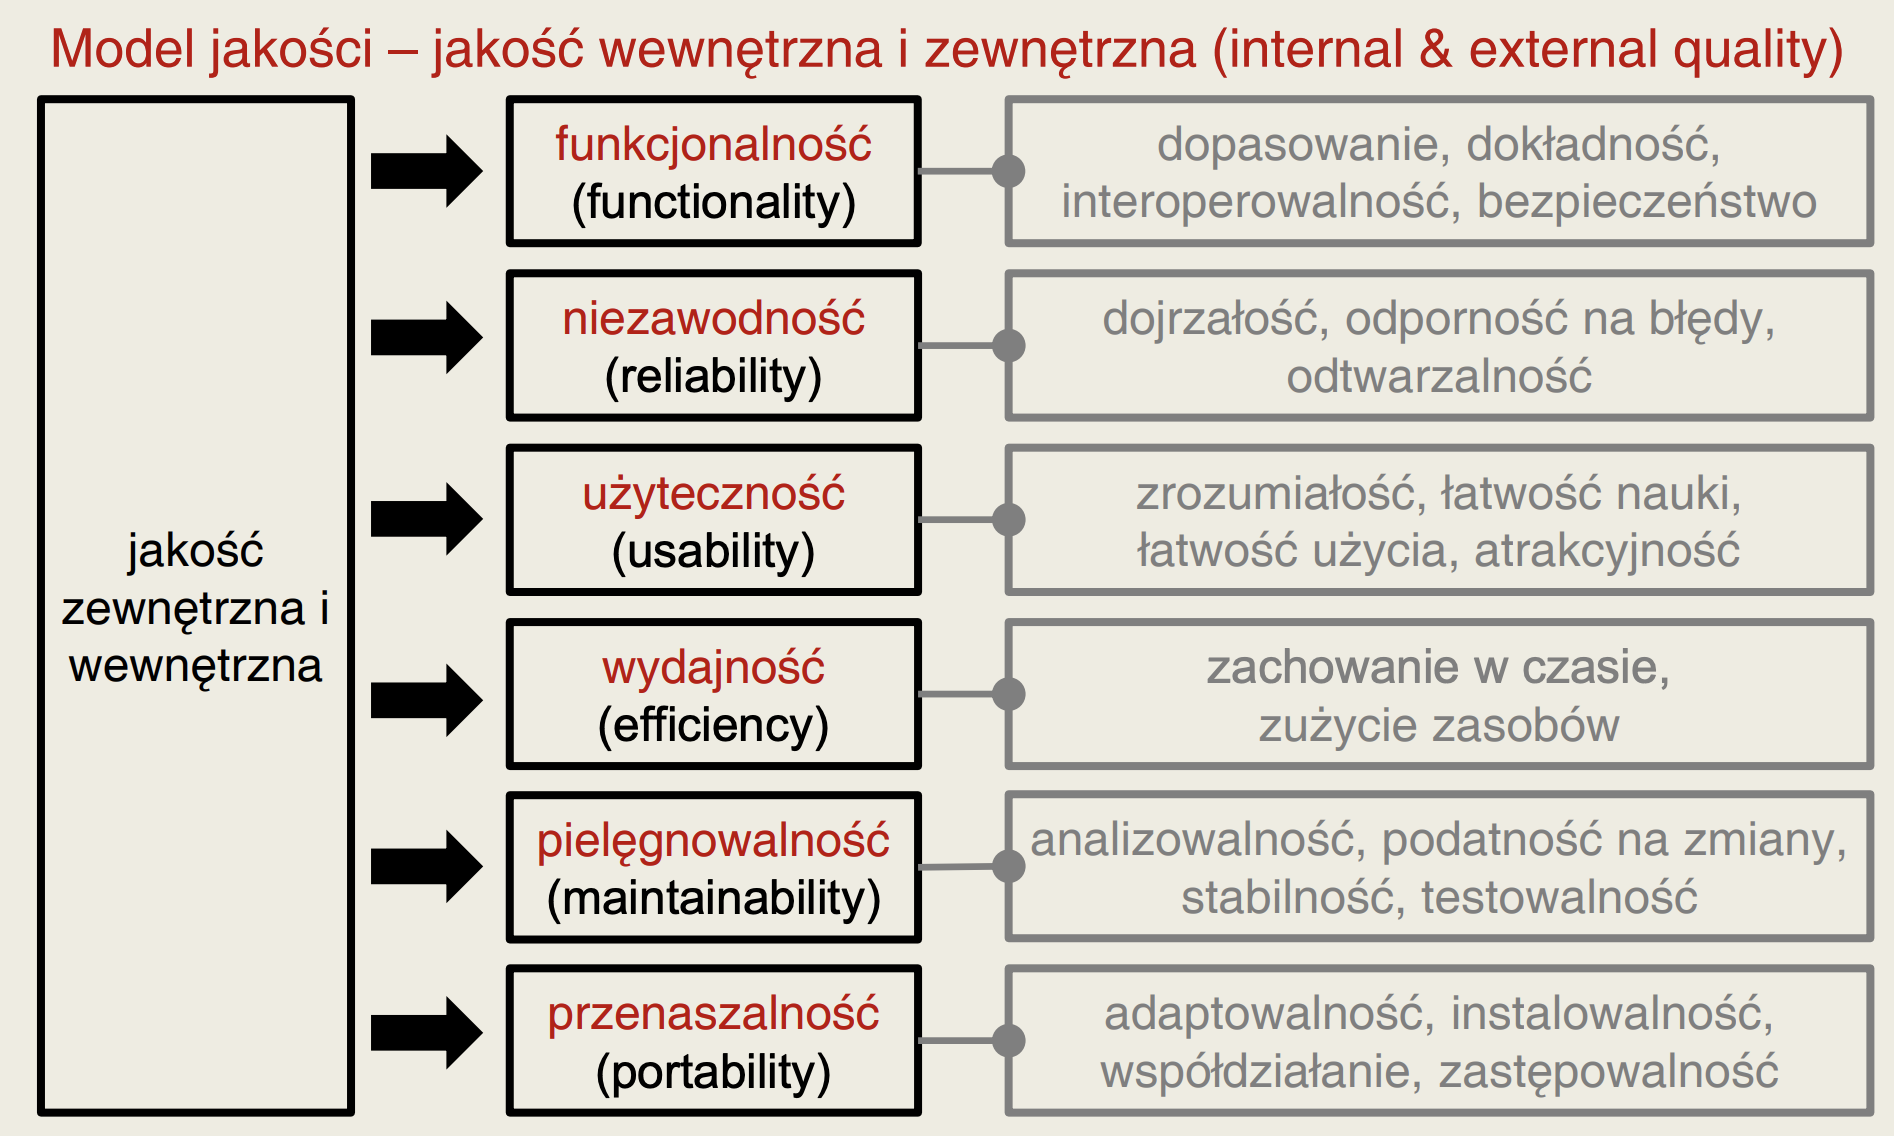
\includegraphics[width=8cm]{ISO9126_1.png}
                &
                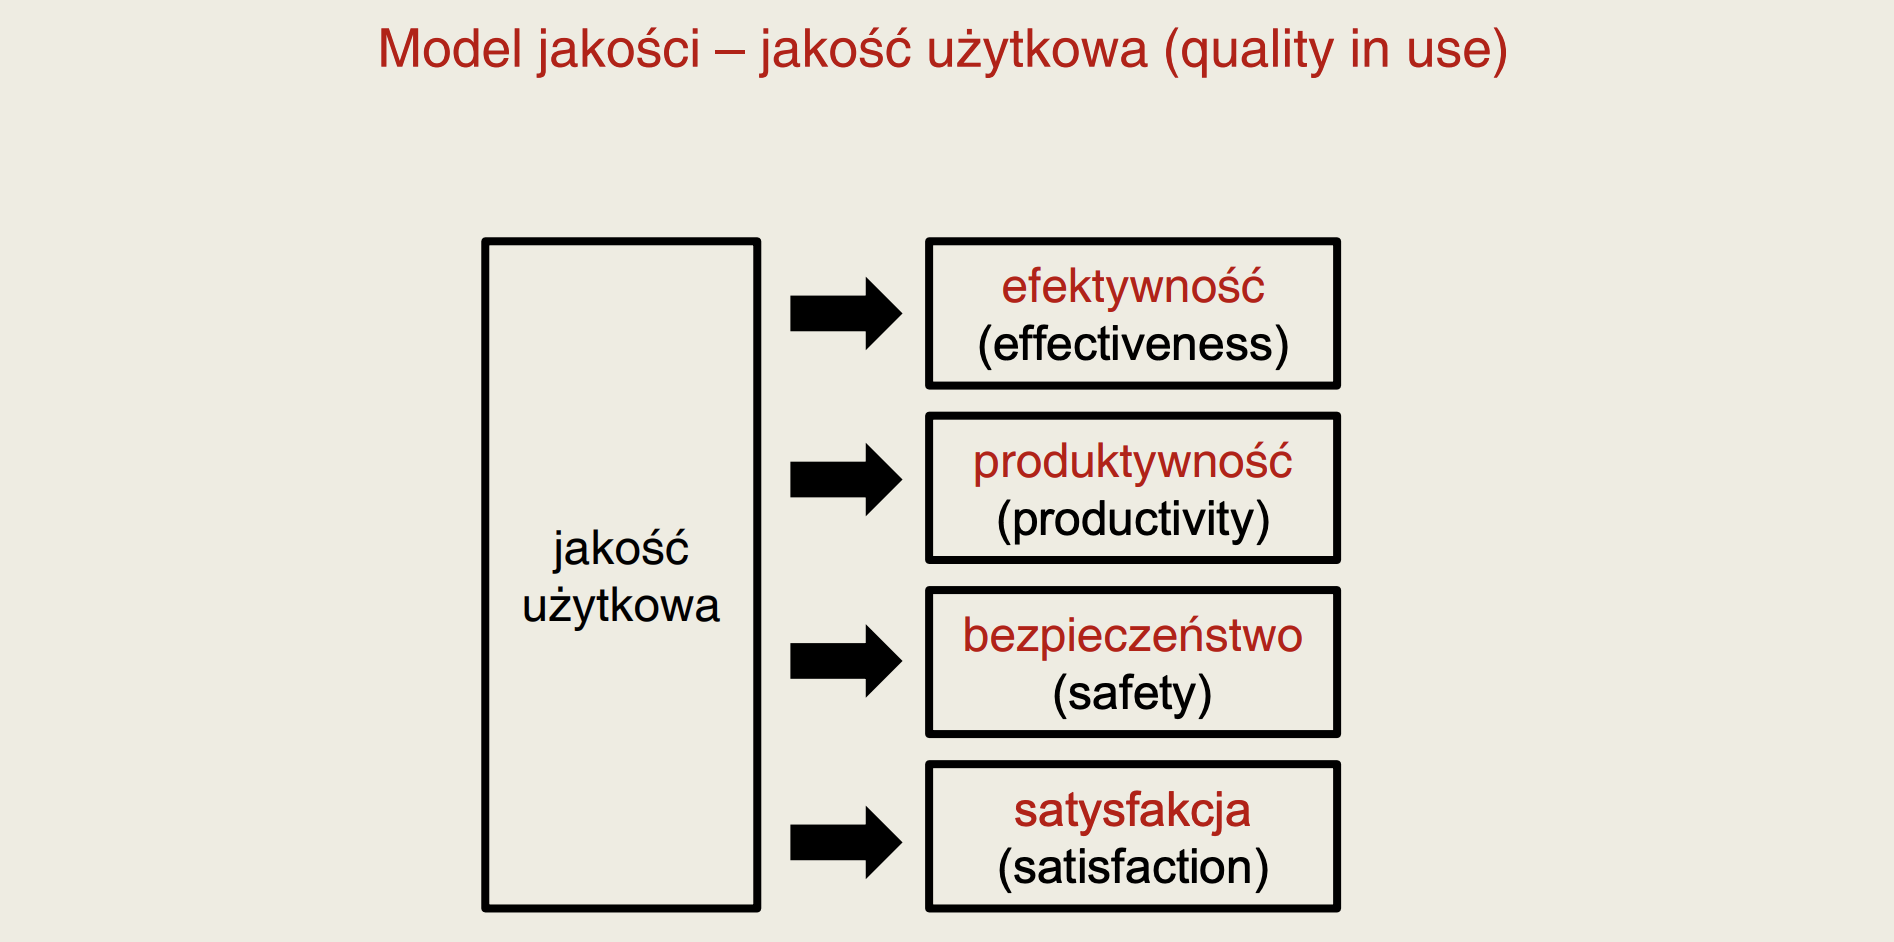
\includegraphics[width=8cm]{ISO9126_2.png}
            \end{tabular}
        \end{center}
    \end{table}

    \subsubsection{Model jakości ISO/IEEE 25000}

    \subsubsection{Niezawodność}

    \textbf{Niezawodność} - \textbf{zdolność} oprogramowania do \textbf{bezbłędnego działania} przez określony czas lub przez określoną
    liczbę operacji. Testy niezawodności wykorzystują \textbf{profile operacyjne}.

    \textbf{Cechy niezawodności}:
    \begin{itemize}
        \item \textbf{dojrzałość} (zdolność do bezawaryjnego działania przy występowaniu usterek)
        \item \textbf{tolerancja na błędy} (np. obsługa wyjątków)
        \item \textbf{odtwarzalność} (zdolność działania po awarii)
    \end{itemize}

    \subsubsection{Bezpieczeństwo}
    \begin{itemize}
        \item Bezpieczeństwo to zbiór atrybutów oprogramowania umożliwiający \textbf{ochronę przed nieautoryzowanym
        dostępem} do programu i danych.
        \item \textbf{OWASP (Open Web Application Security Project)} - obszerna baza zasobów dot. bezpieczeństwa webowego, np.:
        baza ataków, książek i innych materiałów o bezpieczeństwie.
        \item \textbf{SAMM (Software Assurance Maturity Model)} - model pozwalający organizacji zdefiniować i wdrożyć strategię dla zapewnienia bezpieczeństwa,
        dopasowaną do określonych ryzyk.
    \end{itemize}

    \subsubsection{Użyteczność}
    \begin{itemize}
        \item Użyteczność to \textbf{zdolność systemu do bycia zrozumiałym}, łatwym do nauczenia i użycia.
        \item Testowanie \textbf{skupia się na użytkownikach}.
        \item \textbf{Efekty} testowania obserwowane na \textbf{prawdziwych}, końcowych \textbf{użytkownikach}, a nie testerach.
    \end{itemize}

    \begin{table}[H]
        \begin{center}
            \begin{tabular}{p{5cm} p{11cm}}
                \textbf{Podcharakterystyki}
                \begin{itemize}
                    \item Zrozumiałość
                    \item Łatwość nauki
                    \item Łatwość obsługi
                    \item Atrakcyjność
                \end{itemize}
                &
                \textbf{Metryki}
                \begin{itemize}
                    \item \textbf{efektywność} = np. stopień osiągnięcia przez użytkownika celów
                    \item \textbf{wydajność} = ilość zasobów zużytych
                    \item \textbf{satysfakcja} klienta z użytkowania produktu
                \end{itemize}
            \end{tabular}
        \end{center}
    \end{table}



    \begin{table}[H]
        \begin{center}
            \begin{tabular}{| p{8cm} | p{8cm} |}
                \multicolumn{2}{c}{\textbf{TESTOWANIE UŻYTECZNOŚCI}}\\
            \end{tabular}
        \end{center}
    \end{table}
    \begin{table}[H]
        \begin{center}
            \begin{tabular}{| p{8cm} | p{8cm} |}
                \hline
                \multicolumn{2}{|c|}{\textbf{Proces}} \\
                \hline
                \textbf{Formatywne testowanie użyteczności} - przeprowadzane \textbf{iteracyjnie} w
                kolejnych \textbf{fazach projektowania} i prototypowania.
                &
                \textbf{Całościowe testowanie użyteczności} - przeprowadzane \textbf{po implementacji}.
                \\
                \hline
                \hline
                \multicolumn{2}{|c|}{\textbf{Rodzaje}} \\
                \hline
                \textbf{Formalne testowanie użyteczności} - często wymaga uprzedniego \textbf{przygotowania} rzeczywistych
                lub reprezentatywnych \textbf{użytkowników} (dostarczenie scenariuszy zadań, instrukcji).
                &
                \textbf{Nieformalne testowanie użyteczności} - pozwala użytkownikowi \textbf{eksperymentować} z
                oprogramowaniem, aby obserwatorzy ocenili jak trudna dla użytkownika jest praca z systemem. \\
                \hline
                \hline
                \multicolumn{2}{|c|}{\textbf{Walidacja}} \\
                \hline
                \multicolumn{2}{|p{16,5cm}|}{powinna być przeprowadzona \textbf{w warunkach} tak \textbf{bliskich rzeczywistym} warunkom użytkowania
                oprogramowania, jak to tylko możliwe, np. w \textbf{laboratorium użyteczności}.} \\
                \hline
                \hline
                \multicolumn{2}{|c|}{\textbf{Wytyczne (guidelines)}} \\
                \hline
                \multicolumn{2}{|p{16,5cm}|}{są stosowane aby uzyskać \textbf{spójne podejście} do wykrywania i raportowania defektów
                użyteczności \textbf{na wszystkich etapach} cyklu życia.} \\
                \hline
            \end{tabular}
        \end{center}
    \end{table}
    \begin{table}[H]
        \begin{center}
            \begin{tabular}{| p{8cm} | p{8cm} |}
                \hline
                \multicolumn{2}{|c|}{\textbf{Specyfikacja}} \\
                \hline
                \begin{itemize}
                    \item \textbf{Inspekcja, ewaluacja, lub przegląd}
                    \begin{itemize}
                        \item \textbf{Wymagania i specyfikacja}.
                        \item Heurystyczna ocena projektu GUI
                    \end{itemize}

                    \item \textbf{Weryfikacja i walidacja bieżącej implementacji}
                    \begin{itemize}
                        \item Weryfikacja przy pomocy \textbf{przypadków testowych} cech użyteczności
                        zdefiniowanych w wymaganiach
                        \item Walidacja przez scenariusze testowe
                    \end{itemize}
                \end{itemize}
                &
                \begin{itemize}
                    \item \textbf{Dynamiczna interakcja z prototypami}
                    \begin{itemize}
                        \item Praca z \textbf{prototypami} i pomoc deweloperom w ich rozwijaniu
                    \end{itemize}

                    \item \textbf{Ankiety i kwestionariusze}
                    \begin{itemize}
                        \item Zbieranie \textbf{obserwacji} i \textbf{informacji zwrotnej}
                        \item \textbf{SUMI} (Software Usability Measurement Inventory), \textbf{WAMMI} (Website Analysis and Measurement Inventory)
                        – standaryzowane benchmarki
                    \end{itemize}
                \end{itemize} \\
                \hline
            \end{tabular}
        \end{center}
    \end{table}

    \subsubsection{Wydajność}
    \begin{itemize}
        \item \textbf{Zdolność} oprogramowania do \textbf{zapewnienia odpowiedniej efektywności} w działaniu, relatywnie do
        ilości zużytych zasobów
        \item Najczęstsza przyczyna błędów wydajności: \textbf{błędy projektowe}.
    \end{itemize}


    \begin{table}[H]
        \begin{center}
            \begin{tabular}{ p{8cm} | p{8cm} }
                \textbf{Rodzaje testów} wydajności & \textbf{Metryki} dla wydajności \\
                \hline
                \begin{itemize}
                    \item testowanie \textbf{obciążenia}
                    \item testowanie \textbf{warunków skrajnych}
                    \item testowanie \textbf{skalowalności}
                    \item testowanie \textbf{wykorzystania zasobów}
                    \item testowanie \textbf{wytrzymałościowe}
                    \item testowanie \textbf{skokowe}
                    \item testowanie \textbf{niezawodności}
                    \item testowanie \textbf{z aktywnym tłem}
                    \item testowanie \textbf{punktu krytycznego}
                \end{itemize}
                &
                \begin{itemize}
                    \item \% wykorzystania procesora w kluczowym czasie
                    \item dostępna pamięć (RAM, wirtualna)
                    \item top N aktywnych procesów
                    \item liczba przełączeń kontekstów na sekundę
                    \item długość kolejek (procesor, dysk) w danym czasie
                    \item czas podróży pakietu
                    \item czas prezentacji danych klientowi
                \end{itemize} \\
            \end{tabular}
        \end{center}
    \end{table}

    \subsubsection{Pielęgnowalność}
    \begin{itemize}
        \item Pielęgnowalność to \textbf{łatwość modyfikowania oprogramowania}.
        \item Oprogramowanie się nie zużywa, ale staje się \textbf{przestarzałe}.
        \item \textbf{Testowanie pielęgnowalności}
        \begin{itemize}
            \item Zwykle nie przy pomocy skryptów testowych
            \item Większość defektów jest \textbf{niewidoczna dla testowania dynamicznego}
            \item Najlepiej sprawdzają się \textbf{techniki statyczne}
        \end{itemize}
        \item \textbf{Podcharakterystyki pielęgnowalności}
        \begin{itemize}
            \item \textbf{Analizowalność} - łatwość diagnozowania problemów (problem: spaghetti code)
            \item \textbf{Modyfikowalność} - zdolność do wprowadzania zmian (problem: zły standard kodowania)
            \item \textbf{Stabilność} - zdolność do unikania niespodziewanych efektów na skutek zmian (problem: brak kohezji)
            \item \textbf{Testowalność} - łatwość walidacji po wprowadzonej zmianie (problem: zła dokumentacja)
        \end{itemize}
    \end{itemize}

    \subsubsection{Przenaszalność}
    Przenaszalność to \textbf{łatwość, z jaką oprogramowanie może być przeniesione} między środowiskami.
    \begin{itemize}
        \item \textbf{Adaptowalność} – zdolność do adaptacji w innym środowisku bez
        podejmowania akcji innych niż przewidziane w tym celu.
        \item \textbf{Zastępowalność}
        \item \textbf{Instalowalność}
        \item \textbf{Koegzystencja} – zdolność do współistnienia z innym, niezależnym oprogramowaniem dzielącym środowisko
        – np. „przywłaszczenie” standardowego skrótu klawiszowego przez inny program.
    \end{itemize}

\end{document}